\documentclass[11pt]{report}
\usepackage{t1enc,times,a4,t1enc}
\usepackage{graphicx}

\usepackage{listings}
\usepackage{times}
\usepackage{color}
\lstdefinelanguage{VDM++}
  {morekeywords={act, active, fin, req, waiting, abs, all, allsuper, always, and, answer, 
     assumption, async, atomic, be, bool, by, card, cases, char, class, comp, compose, conc, cycles,
     dcl, def, definitions, del, dinter, div, dlmodule, do, dom, dunion, duration, effect, elems, else, elseif, end,
     error, errs, exists, exists1, exit, exports, ext, floor, for, forall, from, functions, 
     general, hd, if, imports, in, inds, infer, init, inmap, input, instance, int, inter, inv, inverse, iota, is, 
     isofbaseclass, isofclass, inv, inverse, lambda, len, let, map, measure, mu,
     mutex, mod, module, nat, nat1, new, merge, 
     munion, not, of, operations, or, others, per, periodic, post, power, pre, pref, 
     private, protected, public, qsync, rd, responsibility, return, reverse,  
     sameclass, parameters, psubset, rem, renamed, rng, sel, self, seq, seq1, set, skip, specified, st, 
     start, startlist, state, static, subclass, subset, subtrace, sync, system, then, thread, 
     threadid, time, tixe, tl, to, token, traces, trap, types, undefined,
     union, uselib, using, values, 
     variables, while, with, wr, yet, RESULT, false, true, nil, periodic pref, rat, real},
   %keywordsprefix=mk\_,
   %keywordsprefix=a\_,
   %keywordsprefix=t\_,
   %keywordsprefix=w\_,
   sensitive,
   morecomment=[l]--,
   morestring=[b]",
   morestring=[b]',
  }[keywords,comments,strings]
\lstdefinelanguage{JavaCC}
  {morekeywords={options, PARSER\_BEGIN, PARSER\_END, SKIP, TOKEN},
   sensitive=false,
  }[keywords]



\parindent 0mm
\parskip\baselineskip

% define the layout for listings
\lstdefinestyle{tool}{basicstyle=\ttfamily,
                      frame=trBL, 
                      showstringspaces=false, 
                      frameround=ffff, 
                      framexleftmargin=0mm, 
                      framexrightmargin=0mm}
\lstdefinestyle{mystyle}{basicstyle=\ttfamily,
                         frame=trBL,
                         showstringspaces=false, 
                        frameround=fttt, 
                         aboveskip=1mm,
                         belowskip=1mm,
                         framexleftmargin=0mm, 
                         framexrightmargin=0mm}

\lstset{style=mystyle}
\lstset{language=VDM++}

\begin{document}

\today

Authors: Peter J\o rgensen

\section*{Overture task suggestions}

The following sub-sections suggest development tasks for the Overture platform.

\subsection*{Quick interpreter improvements}

Currently the error messages given by the Quick Interpreter are not very informative. For example evaluating the expression \texttt{1 + true} yields \textit{``Fatal error''}, wheres the error message would be \textit{``Right hand of + is not numeric. Actual: bool''} when using the VDM editor. It would be useful for the Quick Interpreter to show useful error messages like this. In addition, the Quick Interpreter could be extended to include for instance:

\begin{itemize}

\item A feature for clearing the screen.

\item The possibility writing expressions/statements consisting of multiple lines.

\end{itemize}


\subsection*{Template improvements}

Currently it is possible to use templates for operations, functions cases expressions etc. in the VDM editor by for instance writing \textit{``ope''} followed by the \texttt{Ctrl+space} command. If the user chooses the explicit operation template the following is generated:

\begin{lstlisting}
private operationName : parameterTypes ==> resultType
operationName (parameterNames) == statements;
\end{lstlisting}

Eclipse then assists the user in filling out the template, which is useful for a novice user. The drawback is that every element of the template must be filled out by the user manually. A more experienced user might prefer something which type checks right away. For example, an explicit operation on the form below may require less manual work by the user:

\begin{lstlisting}
public op1 : () ==> ()
op1 () == skip;
\end{lstlisting}

\subsection*{AST structure validation and bug fixing}

The AST provides support for things like finding the nearest ancestor of a node which is a sub class of a given type. For example, it is possible to find the class definition of a given type in the following way:

\begin{lstlisting}
type.getAncestor(SClassDefinition.class)
\end{lstlisting}

Only few Overture plugins use this kind of functionality and there is no proper testing of it. Therefore, it would be a good place to look for bugs. This task suggests writing code that validates the structure of the AST. For example, one could write a visitor checking if the parent of each node has been properly set, i.e. not \texttt{null}. Similarly, other visitors can be made to check if certain properties hold for the AST.

\subsection*{Coverage coloring}

Generated coverage is useful for getting an overview of which parts of a model that have been executed. However, it is possible to find situations where the coverage coloring could be improved. Take for example the generated coverage in figure~\ref{figure:Coverage}.

\begin{figure}[!ht]
\centering
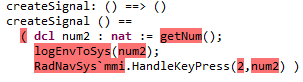
\includegraphics{figures/coverage}
\caption{Coverage of an operation which has not been executed}\label{figure:Coverage}
\end{figure}

It seems strange that only the first ``('' of the block statement is colored. It may be more appropriate not to color the parentheses of a block statement at all. In addition, the \texttt{HandleKeyPress} operation is not colored in red. This task suggests finding problems with the coverage coloring and improving on this feature.

\newpage

\subsection*{Improving robustness of the type checker}

Consider the model below with recursive types.

\begin{lstlisting}
class A
 
types
 
public B = C | nat1; 
public C = B | nat1; 
 
end A
\end{lstlisting}

Using this model we can ask if the union type \texttt{C} is a quote type in the following way:

\begin{lstlisting}
PTypeAssistantTC.isType(C, AQuoteType.class)
\end{lstlisting}

Currently this causes the \texttt{isType} method to call itself recursively until it fails due to a stack overflow error. This task suggests improving the \texttt{isType} method to provide robustness for invocations like this.

\subsection*{Improving the Overture debugging features}

This task suggests improving debugging in Overture by for instance making it possible to:

\begin{itemize}
\item Set break points that will suspend threads at permission predicates.
\item Inspect the value of history counters during debugging.
\item Use the debugging expression evaluator for all kinds of expressions.
\begin{itemize}
\item For example, evaluating the expression \texttt{\textbf{dom} someMap} currently evaluates to ``set'' instead of actually showing what is contained in the set.
\item etc.
\end{itemize}
\end{itemize}

The documentation example model of the POP3 protocol would serve as a good starting point for this task.

\subsection*{RT Trace Viewer improvements}

When executing a VDM-RT model, a series of events are logged and timestamped by a component of the Overture tool, called the RT Logger. During execution, these events are triggered by various actions such as function calls, object creations and thread activations. These events are logged to a text file and a binary file with .rt and .rtbin extensions, respectively. The text file can be inspected by the user using a text editor, while the RT Trace Viewer plugin enables graphical visualization of the binary trace file. This can be used for analyzing timing requirements.

This task suggests a series of nice-to-have features and optimization tasks identified by the plugin authors Martin Askov Andersen, Mads von Qualen and Peter J\o rgensen:

Suggestions for nice to-have-features:
\begin{itemize}
\item A total overview of events for easy scrolling.
\item Make ``Move Next'' and ``Move Previous'' jump to next/previous visible event instead of ``Next'' in terms of time.
%\item Auto draw upon resize
\item The generated conjecture file should be placed in same folder as the .rtbin file.
\item The generated conjecture file should contain additional information which will enable a more precise placement of the conjecture violation circle in the RT log viewer. Preferably by supporting the concepts of relative time and absolute time like in the NextGen data structure. This makes it possible to infer the order of events happening at the same point in time.
\item Maybe the best solution for conjectures would be to integrate the functionality with the NextGen data structure?
\end{itemize}

Optimizations:

\begin{itemize}
\item Change ``jump in time'' model. Currently we draw/parse everything for all CPUs when a new time in the future is selected. Introduce some sort of history model to save object states when they have been parsed. 
\item Refactor TraceFileRunner to move event-parsing (sorting of CPUs etc.) out.
\item Refactor eventhandler base to move conjecture handling out.
\item Cleanup ``update CPU'' hack in TraceFileRunner.
\end{itemize}

\subsection*{Traces }

If you execute traces in the Combinatorial Testing perspective and the test invokes an operation with a failing precondition the verdict is \textit{``nconclusive''}. This is how it should be. What seems strange, is that if you invoke a function with a failing precondition the verdict is \textit{``failed''}. This task suggests changing this so that functions with failing preconditions are considered inconclusive as well.

\end{document}
